\section{Real Clock}\label{sc:realClock}

The real clocks are integrated circuit in electronics with the alternate power source for counting time when the electronics is off, which are used in the systems that needs to keep accurate time. Most of the systems uses crystal oscillator. Because of the clock drift there is a need to synchronize clocks. The two most used algorithms for it is PTP(Precision Time Protocol) and NTP(Network time Protocol) will be described separately below.

\subsection{The need for real clocks}

Why do we need real clocks? Can't we just use the logical ones u just talked about?
Some system needs to know real time(e.g. stock market, bank systems). Logical clocks wont work in this case, because we need precise time oftransactions.
Some system needs to know real time(e.g. stock market, bank systems). Logical clocks wont work in this
case, because we need precise time of transactions.


\subsection{Precision Time Protocol - IEEE 1588}

Precision Time Protocol(PTP) is an open standardized protocol for synchronizing time, published by the IEEE under the numerical value of 1588. PTP is one of the more precise synchronization standards in general use and was designed to allow for high precision while being easy to install and requiring minimal resources. PTP is a master slave protocol with the master holding a correct clock value, the master will inform the slave of the time.

\noindent The protocol is built from two procedures that occur in parallel, first a syntonization is run to get the clocks running at the same speeds, and secondly a calculation of the slave's offset from the master. 
\begin{enumerate}
\item Send periodic messages to the slave allowing the slave to adjust it's clock speed to match.
\item Calculate the slave's offset from the master and the delay introduced during transmission. As a side effect of these calculations the clock value is set as t - offset.
\end{enumerate}

\noindent This split in traffic and periodic maintenance is well suited to packet switched networks as there is no need for dedicated lines of communication and the line can easily be shared with other applications. A second benefit of the small resource footprint of PTP is that it allows a single server to synchronize with multiple slaves, while being synchronized in turn. The system is infinitely hierarchical, with masters having the ability to simultaneously being slaves to a different master, this means that the protocol can be infinitely scaled up with relatively small overhead.

\noindent PTP is excellent to use in systems where extremely high precision is required  inside the real-time domain. Especially in applications for scientific, measurement and control systems.

\subsection{NTP - Network time Protocol}

NTP was design by David L. Mills and it is operational since before 1985. It is one of the oldest protocol in
current use. The core principal of the protocol is server-client communication. In the stratum 0 is located
most accurate timekeepers (e.g. GPS, radio clock, etc.). These timekeepers are directly interfacing to the
stratum 1 servers, also between same level stratum severs can be interface to each other as shown in \ref{fig:NTP}.

\begin{figure}[H]\label{}
	\centering
	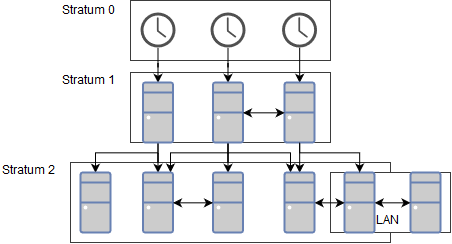
\includegraphics[scale=0.4]{synchronization/fig/NTP.png}
	\caption{An DFA that accepts any input that contains two '1' symbols in a row}
	\label{fig:NTP}
\end{figure}

\noindent Pros of network time protocol is that the client can be connected to more then one severer to get time, itis cheaper to develop NTP then PTP. Has feature called "Insane Time" which prevents synchronization witha server who is 1024 seconds apart.

\noindent Cons requires at lest one interface through wide area network which leads to security issues. Below stratum
15 devices are held unsynchronized.
Cons requires at lest one interface through wide area network which leads to security issues. Below stratum15 devices are held unsynchronized.
